\chapter{Limpeza e Manutenção}

\section*{Sistema eletroeletrônico}
\par Para a limpeza e manutenção dos componentes eletrônicos e placas de circuito impresso recomendasse a utilização de Álcool Isopropílico para a sua limpeza por possuir a miníma ou nenhuma porcentagem de água evitando a oxidação dos componentes e trilhas das placas e pincel antiestática para assegura o pleno funcionamento das placas com o decorrer do tempo. Para limpeza é necessário os seguintes materiais: 
\begin{itemize}
    \item Álcool Isopropílico
    \item Pinça
    \item Algodão
    \item Pincel antiestática
\end{itemize}

\par Passos:
\begin{itemize}
    \item Limpe as placas de circuito impresso com cuidado e passando o pincel antiestática sobre todo comprimento da placa como na figura \ref{fig:pincel} para a remoção da camada de partículas sobre a placa.
    \begin{figure}[H]
  \centering
  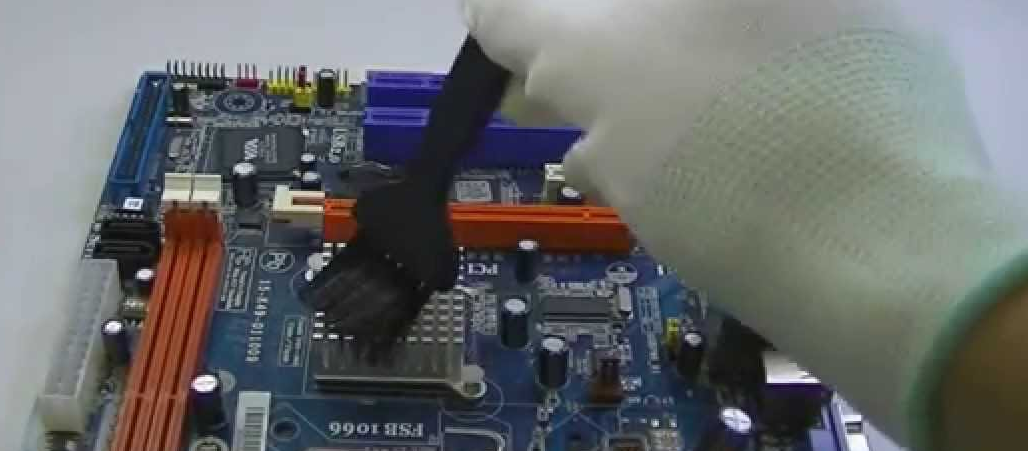
\includegraphics[width=\textwidth]{Figuras/pincel.png}
  \caption{Limpeza com pincel.} 
  \label{fig:pincel}
\end{figure}
\item Para a limpeza é necessário pegar um pedaço de algodão com a pinça e colocar Álcool Isopropílico nele, limpar as conexões de solda e as tarinhas de maneira cuidadosa evitado danos a placa. 
    \begin{figure}[H]
  \centering
  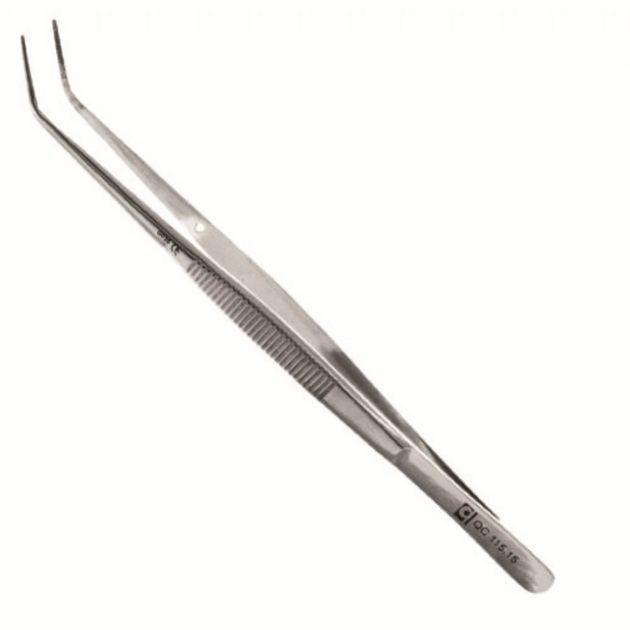
\includegraphics[scale=0.2]{Figuras/Pinca-para-Algodao-Quinelato.jpg}
    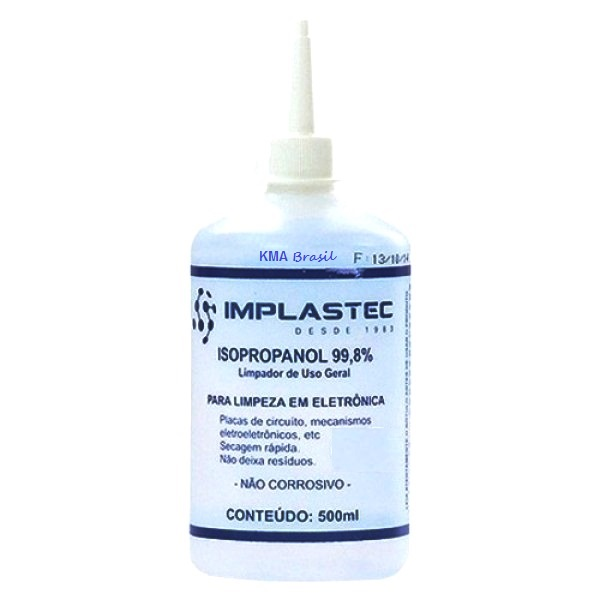
\includegraphics[scale=0.3]{Figuras/alcool-500ml-1-90045.jpg}
      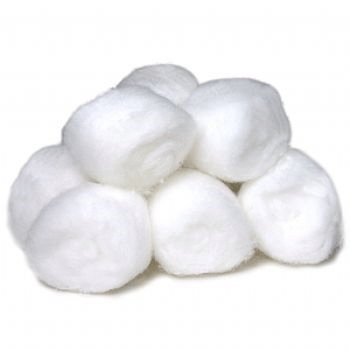
\includegraphics[scale=0.3]{Figuras/Bolas-de-Algodao.png}
  \caption{Limpeza com Álcool Isopropílico.} 
  \label{fig:alcoo}
\end{figure}

    \end{itemize}

\section*{Sistema hidráulico}

\par As partes do sistema de abastecimento que entrarem em contato com o propelente líquido, devem ser ao final do uso, expostas ao ar ambiente para entrar em contato com o oxigênio e evaporar os resquícios que possam existir ainda dentro do sistema. 

\par As válvulas e mangueiras utilizadas, não devem entrar em contato com outras substâncias que não sejam as indicadas, para o uso do sistema. Porém caso aconteça da tubulação entrar em contato com alguma substância externa, recomenda-se o uso de um pano macio e sem fiapos levemente umidificado e bem torcido, ou o auxilio de hastes de algodão para a limpeza interna.

\subsection*{Sistema de atuação}

\par O sistema de atuação é feito de uma case da aço SAE 1020, por isso para limpar o mesmo deve-se seguir as recomendações de limpeza e conservação de aço carbono. Assim a limpeza deve ser feita com um pano úmido, sabão neutro e esponja de nylon. Pelo fato do sistema possuir um motor dentro dele não é recomendado a lavagem da case em contato direto com a água por causa dos riscos de danificação do sistema. Após a limpeza seque bem a parte externa com um pano macio, seco e limpo, além de garantir que toda a umidade foi eliminada, pois aço carbono corre o risco de corroer caso não fique bem seco.

\par Deve-se atentar ao fato de que a válvula esfera é presa por dois mancais dentro da estrutura de atuação, e os mesmos devem ser lubrificados periodicamente de acordo com as especificações do fabricante.

\section*{Estrutura}

\par A seguir são apresentadas algumas dicas gerais para a limpeza e manutenção do seu produto.

\begin{itemize}
    \item Não utilize materiais de limpeza inflamáveis ou tóxicos, a não ser quando recomendado.
    \item Não faça qualquer manutenção ou limpeza no produto com ele conectado a rede elétrica ou com as baterias carregadas.
    \item Limpe as partes interiores usando um pano macio ou hastes de algodão de preferência.
    \item Se a estrutura for exposta a algum tipo de substância líquida ou química, limpe-o com um pano macio e sem fiapos.
\end{itemize}

\subsection*{Partes em MDF}

\par A estrutura das maletas são feitas em MDF, porém apesar de seu exterior revestido, seu interior ainda está sujeito ao contato com o ambiente externo. Por isso para limpar o interior do mesmo alguns cuidados devem ser seguidos, primeiramente o MDF cru não deve entrar em contato com a água, pois sua composição não é hidrofóbica.

\par Sabendo-se disso deve-se seguir as recomendações de limpeza apresentadas, onde a limpeza deve ser feita com um pano úmido e bem torcido, caso aja manchas na superfície pode-se usar uma substância a base de álcool ou sabão neutro para a limpeza. Se necessário seque com um pano seco e limpo.

\subsection*{Partes Emborrachadas}

\par A limpeza de materiais emborrachados, segue as mesmas diretrizes apresentadas anteriormente para o MDF, atentando-se ao fato de que não é recomendado o uso de álcool para a limpeza deste. Para uma secagem adequada recomenda-se deixar a estrutura ao ar livre até a secagem por completo do material. 

\par Borrachas são sensíveis a mudanças ambientais e podem ressecar e quebrar com o tempo, para que isso não ocorra é recomendado o uso de uma solução hidratante para borrachas que deve ser aplicada ao menos duas vezes ao ano.

\subsection*{Partes em PLA}

\par O PLA é um tipo de plástico desenvolvido para a impressão 3D, por isso para sua limpeza deve-se tomar as medidas de limpeza de um plástico comum. De forma que a limpeza do mesmo pode ser feita usando-se um pano úmido e sabão neutro, caso necessário pode-se fazer uso de uma esponja domestica para tirar manchas e sujeiras. 

\par Está também não deve entrar em contato direto com a água para não danificar as PCI's que comportam.

\par O PLA é um material solúvel a acetona então é muito importante para a integridade da estrutura que ela não seja exposta a esta substância.